\documentclass{beamer}

\mode<presentation>
{
  \usetheme{Madrid}      % or try Darmstadt, Madrid, Warsaw, ...
  \setbeamertemplate{navigation symbols}{}
  \setbeamertemplate{caption}[numbered]
} 

\colorlet{beamer@blendedblue}{black}

\usepackage[french]{babel}
\usepackage[utf8x]{inputenc}
\usepackage[T1]{fontenc}
%\usepackage[squaren,cdot]{SIunits}
\usepackage{graphicx}
\usepackage{listings}

\graphicspath{}

\logo{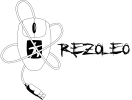
\includegraphics[height=0.8cm]{rezoleo.png}\vspace{10pt}\hspace{20pt}}
\title{Introduction aux réseaux}
\author{LEDER "Ziman" Simon}
\institute{Rezoleo\\}
\date{\today}

\begin{document}
	
	\maketitle

	\begin{frame}
		\frametitle{Sommaire} 
		\tableofcontents
	\end{frame}

\section{Définition}
	
	\begin{frame}{Définition}
		Un réseau informatique est un ensemble d'\textbf{équipements} reliés entre eux pour échanger des informations entre un ou plusieurs ordinateurs. \\
		\begin{itemize}[<+->]
			\item Des ressources périphériques tels les imprimantes, lecteurs, scanners, caméra IP, Domotique
			\item Des données tels que les fichiers et les logiciels 
			\item La gestion des comptes utilisateurs
			\item Les ponts entre deux sites d’entreprise (VPN) 
			\item Le courrier électronique
			\item L’accès au World Wide Web
			\item Le transfert de fichiers (ftp)
			\item L’accès à distance (telnet, ssh) la prise de contrôle à distance
		\end{itemize}
	\end{frame}

\section{Historique}

	\begin{frame}{Historique}
		\begin{center}
			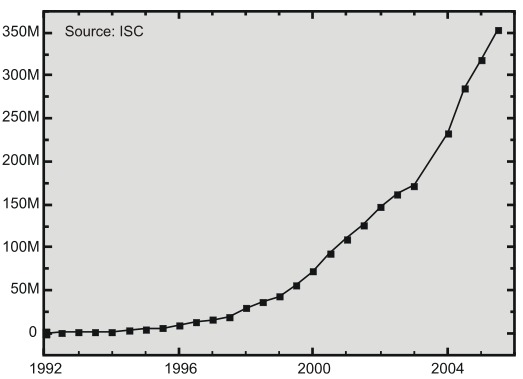
\includegraphics[scale=0.7]{Utilisation.png}
		\end{center}
	\end{frame}

	\begin{frame}{Historique}
		\begin{itemize}[<+->]
			\item 1969 - 1978 : ARPANET
			\item 1983 : Protocoles TCP/
			\item 1984 : 1000 ordinateurs connectés
			\item 1995 : IPv6
			\item 2014 :
 		\end{itemize}
	\end{frame}

	\section{Type de réseaux}

	\begin{frame}{Type de réseaux}{structure physique}
		\begin{itemize}
			\item Les supports de communication (câbles, fibres, faisceaux, liaisons physiques, lignes de transmission, médium, etc.)
			\item Les équipements d’interconnexion (noeuds, routeurs, ponts, passerelles, etc.)
			\item Les équipements terminaux (ordinateurs, stations, serveurs, périphériques, machines hôtes, stations, etc.)
		\end{itemize}
	\end{frame}
	
	\begin{frame}
		\begin{center}
			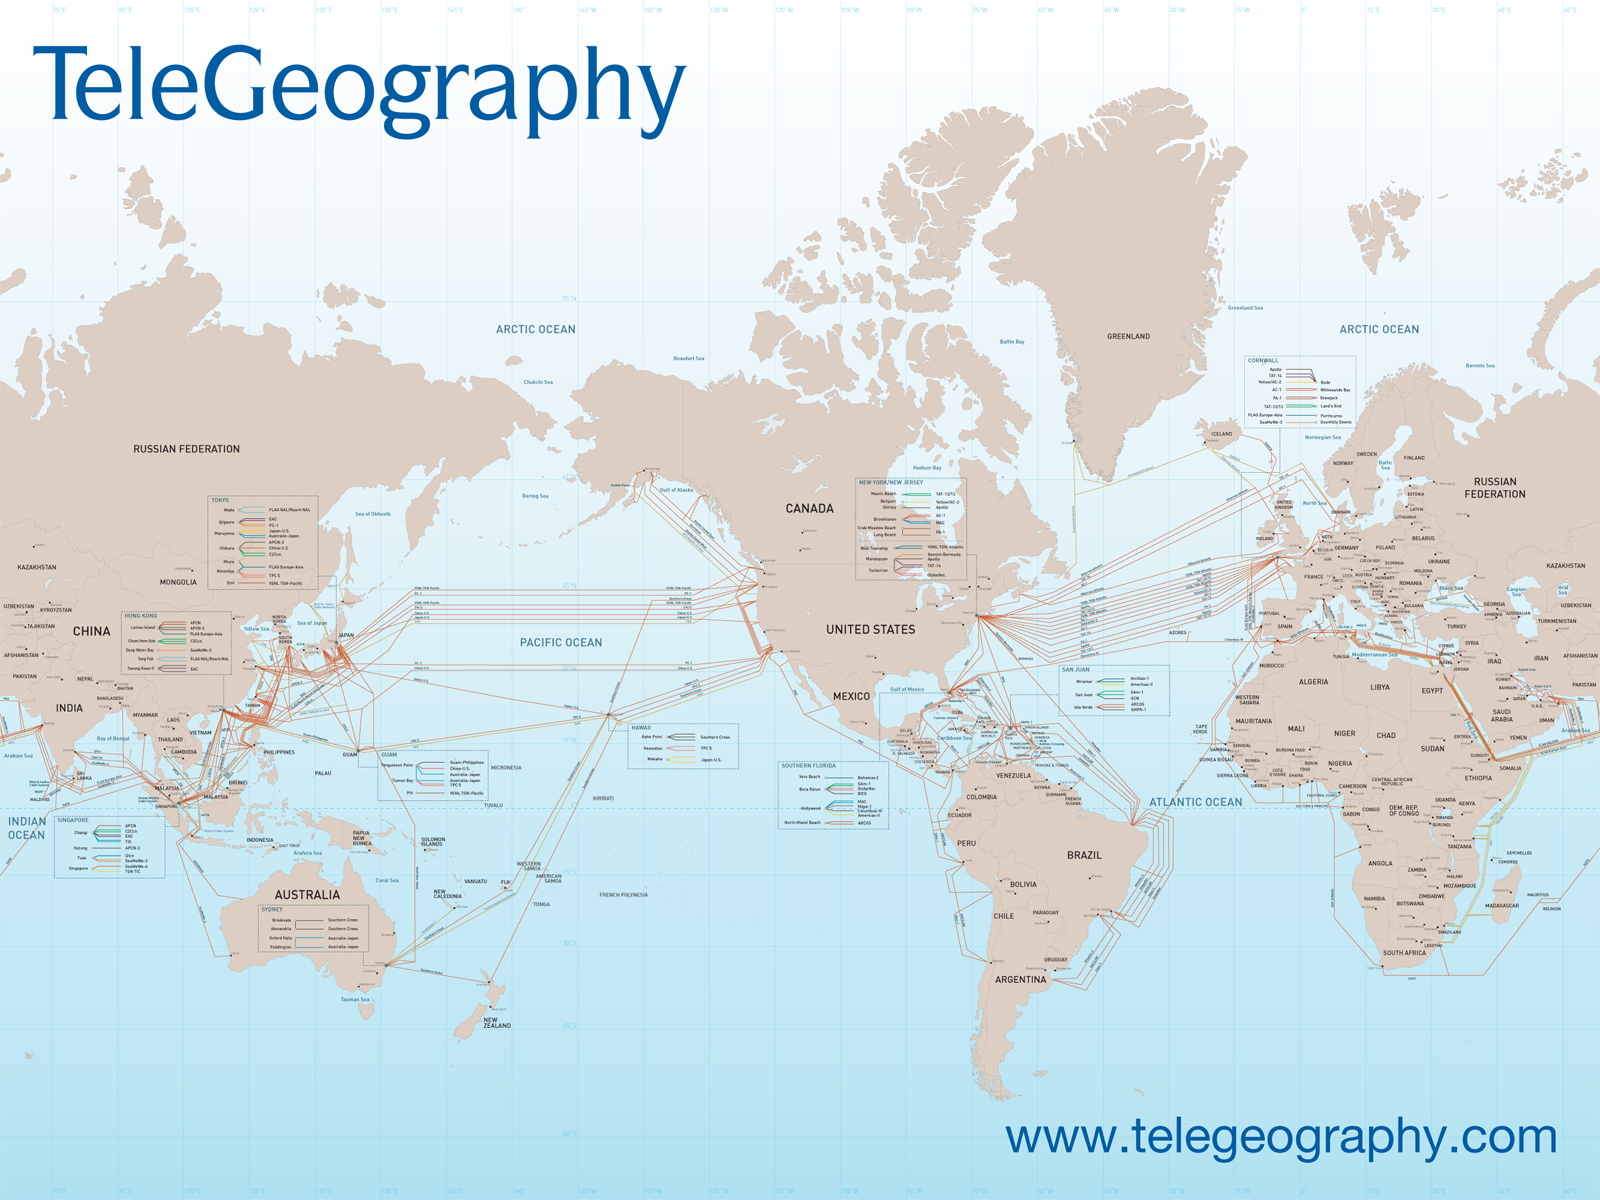
\includegraphics[scale=0.35]{Carte.jpg}
		\end{center}
	\end{frame}

	\begin{frame}{Type de réseaux}{Classes de réseaux}
		\begin{itemize}
			\item PAN (Personal Area Network)
			\item LAN (Local Area Network)
			\item MAN (Metropolitan Area Network)
			\item WAN (Wild Area Network)
			\item Autres réseaux (DAN, SAN)
		\end{itemize}
	\end{frame}

\end{document}